\documentclass[a4paper, dvipdfm]{article}
\usepackage{graphicx}

\setlength\oddsidemargin{-.25 in}
\setlength\textwidth{6.75 in}
\setlength\topmargin{-.5 in}
\setlength\textheight{9.75 in}

\makeatletter
\def\maketitle{%
  \null
  \thispagestyle{empty}%
  \vfill
  \begin{center}\leavevmode
    \normalfont
{\LARGE \@title\par}%
    \vskip 1cm
{\Large \@author\par}%
    \vskip 1cm
{\Large \@date\par}%
  \end{center}%
  \vfill
  \null
  \cleardoublepage
}
\makeatother

\pagestyle{myheadings}
\markboth{KiCAD 3D VRML Models, Python bindings}{}


\title{TUTORIAL\\
KiCAD 3D VRML Models\\
and\\
Python Bindings}
\date{Version 0.9\\
12 Apr 2014}
\author{Dr. Cirilo Bernardo}

\begin{document}

\maketitle

% Revision history, if desired
%\pagenumbering{roman}
%\textbf{\Large{Revision History}}
%\vspace{1 ex}
%
%\begin{tabular}{|l|l|p{4.5in}|}
%\hline
%\textbf{Revision} & \textbf{Date} & \textbf{Comments}\\
%\hline
%RevA.1 & 2012-11-12 & Initial draft\\
%\hline
%\end{tabular}
%
%\clearpage

% start main numbering sequence
\setcounter{page}{1}
\pagenumbering{arabic}

\section{Introduction}
The Kicad 3D Models project aims to produce high-quality parametric models for use
with KiCAD.  Initially these will be VRML2.0 models for use in the KiCAD 3D Viewer
but as the Free-CAD project matures, Free-CAD solid models will also be added with
the intention of providing a means of generating a solid model of the board to aid
users with their mechanical integration requirements.

This document describes the installation and use of the Python modules for generating
VRML models from existing parametric models as well as how to use the existing
parameterized features from the toolbox to create new parametric models within Python.

For an introduction to using VRML2.0 with KiCAD, see the document \emph{kicad\_3d\_vrml.pdf}
``Tutorial: VRML2.0 and KiCAD'' and references therein.

This document assumes the user is familiar with the VRML2.0 specification and the
current limitations of the KiCAD 3D viewer which restrict the VRML features used
in the 3D models. The user is also assumed to have a basic familiarity with
the GNU compiler and the Python interpreter.

This tutorial is aimed at users with a GNU/Linux system since the source code has
been developed on such a system; users with experience on other systems are
encouraged to make appropriate adjustments to the source code and build tools and
to report results to the author via the project website (http://kicad3dmodels.sourceforge.net).

To view the VRML models, use a viewer such as \verb#whitedune# on Linux or \verb#Cortona3D#
on MSWindows.

\section{Installation}
The current requirements for installation of the Kicad 3D parametric models are:
\begin{itemize}
\item git version 1.7 or later (earlier versions may work)\\
\item Kicad3DModels source code\\
\item GNU C++ compiler\\
\item CMake version 2.8 or later (earlier versions may work)\\
\item Python version 2.6 or later\\
\item Boost::Python version 1.49 or later (earlier versions may work)\\
\end{itemize}

To retrieve the source code via git, change to your preferred working directory
then invoke git to create the project's subdirectory:

\verb#git clone git://git.code.sf.net/p/kicad3dmodels/code kicad3d#

Change to the top level project directory:

\verb#cd kicad3d#

The project uses the CMake build tool and each subdirectory contains a
\verb#CMakeLists.txt# file with instructions for CMake. Since the 
instructions to build the Python bindings depends on the specific setup
of your system, you will need to edit the file \verb#src/py/CMakeLists.txt#
and check the following:

\verb#SET(ENV{BOOST_ROOT} "/usr/lib")# Set the path to your BOOST installation

\verb#SET(PYTHON_INCLUDE "/usr/include/python2.7")# Set the path to the header
files for the version of Python you wish to use.

\verb#SET(PYTHON_VERSION python2.7)# Set to the version of Python you wish to use.

\verb#find_package(Boost 1.49 EXACT REQUIRED COMPONENTS python)# Set the BOOST version
to the version installed on your system.

Once those changes are made we should be ready to configure and build the tools.
To keep the source tree free of temporary build files, we will create a build
directory in the top level project directory (\verb#kicad3d#) then build and install
the files:

\begin{verbatim}
mkdir build
cd build
cmake ..
make install
\end{verbatim}

The various tools and libraries will be built; executable files will be installed within
the \verb#scripts/bin# directory in the project tree and the Python modules will be
installed within the \verb#scripts/lib# directory. The Python modules will have names
such as \verb#libkc3d.so# while Python expects names such as \verb#kc3d.so#; you may work
around this issue by renaming the files or by using symlinks, for example:

\begin{verbatim}
cd scripts/lib
ln -s libkc3d.so kc3d.so
ln -s libkc3dconn.so kc3dconn.so
ln -s libkc3ddiode.so kc3ddiode.so
ln -s libkc3ddip.so kc3ddip.so
ln -s libkc3dres.so kc3dres.so
\end{verbatim}

This software is in its early development stages so it is recommended that the modules
remain in the \verb#scripts/lib# directory. To check that everything is fine, set the
\verb#PYTHONPATH# environment variable to include the \verb#scripts/lib# directory;
if the environment variable is not set, one way to set its value is to change to the
\verb#script/lib# directory and then execute the command \verb#export PYTHONPATH=${PWD}#.
We should now be able to load the modules from within Python:

\begin{verbatim}
python
Python 2.7.3rc2 (default, Apr 22 2012, 22:35:38) 
[GCC 4.6.3] on linux2
Type "help", "copyright", "credits" or "license" for more information.
>>> import kc3d
>>> import kc3dconn
\end{verbatim}

\section{Quick Example}
\label{sec:quick-example}
In this brief example we will invoke a single parametric model to
build a variety of 6x2 DIL headers as a demonstration of the
flexibility of parametric models.

For consistency in the appearance of materials in the models, material
appearances are defined in files within the directory \verb#mcad/colors#.
For the convenience of this exerice and all future exercises in this
tutorial, we will create models from the directory \verb#mcad/test#;
create the test directory and change to it. Ensure that the PYTHONPATH
had been set as discussed in the section on installing the software.
All future examples in this tutorial will assume that the working
directory is \verb#mcad/test#.
Run Python and execute the following Python commands (ignore lines
beginning with `\#' - these are merely code comments):

\begin{verbatim}
# load the tools
import kc3d
import kc3dconn
from kc3d import *
from kc3dconn import *

# instantiate necessary objects
out = ofstream()
hdr = Genhdr()
tx = Transform()
# set the scale to 1/2.54 so that the VRML units correspond to
# the 0.1 inch used by KiCAD.
tx.setScale(0.3937)

# create a male 6x2 header with square pins 8mm high, 2.54mm pitch, and beveled case
SetupVRML("testhdr_MS_6x2_8mm.wrl", out)
hdr.setColors("../colors/black.mat", "../colors/gold.mat", "../colors/gold.mat", "../colors/tin.mat")
hdr.setCase(6, 2, 2.54, 2.54, 2.72, 0.72, True, 0.3)
hdr.setPins(True, True, True, -1, -1, 2, 10, 0.64, 0.64, 0, 0, 0, 0, 0.3, 0.8, 4, 0)
hdr.build(tx, "HDR_MALE_SP_6x2_8MM", out, 0)
out.close()

# create a female 6x2 header with square pins, 8mm high beveled case, 2.54mm pitch
kc3d.SetupVRML("testhdr_FS_6x2_8mm.wrl", out)
hdr.setColors("../colors/black.mat", "../colors/tin.mat", "../colors/gold.mat", "../colors/black.mat")
hdr.setCase(6, 2, 2.54, 2.54, 8, 0.72, True, 0.3)
hdr.setPins(True, True, False, -1, -1, 2, 10, 0.64, 0.64, 1.6, 1.09, 0, 0, 0.3, 0.8, 24, 0.5)
hdr.build(tx, "HDR_FEMALE_SP_6x2_8MM", out, 0)
out.close()

# create a female 6x2 header with round pins, 8mm high beveled case, 2.54mm pitch
kc3d.SetupVRML("testhdr_FR_6x2_8mm.wrl", out)
hdr.setCase(6, 2, 2.54, 2.54, 8, 0.72, True, 0.3)
hdr.setPins(False, False, False, -1, -1, 2, 10, 0.64, 0.64, 1.6, 0.84, 1.32, 1.2, 0.3, 0.8, 24, 0.5)
hdr.build(tx, "HDR_FEMALE_RP_6x2_8MM", out, 0)
out.close()
\end{verbatim}

Exit the python interpreter and inspect the model files with a VRML viewer.
This is only a very brief introduction to a parametric model. For this
particular model (\verb#Genhdr#), many parameters can be changed to produce
a different model - for example, the number of rows or columns can be changed
and the case can be plain with no bevel. The model only produces vertical
headers with straight pins but the model itself relies on other components
which describe the shape of a pin and the shape of the case; these more
basic components can be used to create models for generating 90-degree
headers, SMD headers, and so on.

% XXX - put in pretty pictures


\section{KC3D: The VRML Toolbox}
As mentioned in the previous section, parametric models may be built on more
basic components which can be used in a variety of models. This section
describes these basic components and the details of their parameters. The
basic models are organized into the \verb#kc3d# module. As with many Python
modules, interactive information can be displayed about the module and
its components, for example:

\begin{verbatim}
import kc3d
help("kc3d")
help("kc3d.Polygon")
help("kc3d.Circle")
\end{verbatim}

This section aims to present the details of each component of the kc3d module
in a more intelligible fashion, but while working within the Python interpreter
the built-in information is a very helpful tool.


\subsection{kc3d.ofstream()}
This object is a simple wrapper for the C++ std::ofstream which is used as
a parameter to all routines which write data to a file. The exposed methods
are as follows:

\textbf{kc3d.ofstream.open(filename)} : opens the file with the given filename.

\textbf{kc3d.ofstream.close()} : closes the file.

\textbf{kc3d.ofstream.good()} : returns 1 if the file stream is in a good state
and 0 if there are errors.

\textbf{kc3d.ofstream.is\_open()} : returns 1 if a file is currently open.

\subsection{kc3d VRML File Operations}
There are a number of methods which can be called directly from the
kc3d module to operate on VRML files.

\textbf{kc3d.SetupVRML(filename, file)} : Open a VRML file with the given
filename and write the header information. The argument \textbf{file}
is an object of type \textbf{kc3d.ofstream()}.  Return values are
0 for success and -1 for failure.

\textbf{kc3d.SetupXForm(name, file, tabs)} : Creates the opening
text for a VRML Transform block.  The \textbf{name} is the name
of the transform, \textbf{file} is a file which was previously opened
via a call to \textbf{SetupVRML}, and \textbf{tabs} is the
formatting indentation level. Return values are 0 for success and
-1 for failure.

\textbf{kc3d.CloseXForm(file, tabs)} : Close a VRML Transform block previously
opened by a call to \textbf{SetupXForm}. Return values are 0 for
success and -1 for failure.

\textbf{kc3d.SetupShape(color, reuse, file, tabs)} : Creates the
opening text for a VRML Shape block; the text includes the 
appearance specification. The argument \textbf{color} is of
type \textbf{kc3d.VRMLMat} and it must already have loaded its
color definition from a file. If \textbf{reuse} is 1, the
Shape block will assume that the material appearance had
previously been written to the VRML file and will employ the
VRML USE directive to reuse the previous definition.
The argument \textbf{file} is an open VRML file. Return values
are 0 for success and -1 for failure.

\textbf{kc3d.CloseShape(file, tabs)} : Closes a VRML Shape block previously
opened via \textbf{SetupShape}. In a typical sequence of operations
a Shape block is opened and a geometry and coordIndex block is written
to describe a surface. Multiple Shape blocks are written to a
Transform block to describe the entire component. Return values are
0 for success and -1 for failure.

\textbf{kc3d.WriteCoord(*X, *Y, *Z, np, file, tabs)} : \textbf{*X},
\textbf{*Y}, and \textbf{*Z} are pointers to arrays containing the
coordinates of vertices and \textbf{np} is the number of vertices.
This method writes the series of coordinate points to a
coordinate block. Return values are 0 for success and -1 for failure.

\textbf{kc3d.SetupCoordIndex(file, tabs)} : Create the opening text
of a VRML coordIndex block. After opening such a block, the user
must write a list of indices defining each facet to be rendered.
Return values are 0 for success and -1 for failure.

\textbf{kc3d.CloseCoordIndex(file, tabs)} : Closes a coordIndex
block. Return values are 0 for success and -1 for failure.

\subsection{kc3d.Material() and kc3d.VRMLMat()}
The \textbf{Material} class is the representation of the VRML2.0 material
appearance as described in individual files in the project's \verb#mcad/colors#
directory. The base class is meant to hold the basic data while derived classes
implement input and output functions specific to the class of 3D models such
as VRML, Free-CAD, etc. Only the \textbf{Load} function has been exposed to
Python and it has the following form:

\textbf{Material.Load(filename)}: where the filename is the path to a
material definition file. Return values are 0 for success and -1 for failure.

The \textbf{VRMLMat} class is derived from \textbf{Material} and implements
the \textbf{Write} routine to write a VRML2.0 material appearance block to
a file:

\textbf{VRMLMat.Write(file, tabs, mainblock)}: where \textbf{file} is an open
output file of type \textbf{kc3d.ofstream()}, \textbf{tabs} is an integer
specifying the formatting indentation level, and \textbf{mainblock} is a boolean
which controls the content of the output information; if the value is 0 then
a material block appropriate for inclusion in a VRML Shape block is generated,
otherwise a material block appropriate for inclusion in the main VRML body
is generated.  Return values are 0 for success and -1 for failure.

For more information on material specifications, see the VRML2.0 specification.
The use of material specification files is encouraged to promote uniformity of
appearance between related classes of models created by different users or by
a single user at a different time. Below are the contents of a material
specification file for the appearance of the glass envelope of a DO-35 packaged
axial glass encapsulated diode:

\begin{verbatim}
# Clear glass

name: glass_clr
diffuse: 0.3 0.3 0.3
emissive: 0 0 0
specular: 0.3 0.3 0.3
ambient: 1
transparency: 0.6
shininess: 1
\end{verbatim}

\subsection{kc3d.Quat()}
The \textbf{Quat} class is the representation of a basic quaternion. It supports
multiplication and division by a scalar and addition and subtraction of quaternions
and scalars. The quaternion can be normalized by invoking the method \textbf{normalize()}
or the vector component alone can be normalized via a call to \textbf{vnormalize()}.
The individual components w, x, y, and z are publicly exposed. The cross product
and angle of two vectors can be calculated by \textbf(cross(vector\_b)) as demonstrated
in the script below. The cross product assumes a right-handed coordinate system; if
you are using a left-handed coordinate system you must multiply the pseudovector
coefficients by the appropriate unit vector coefficients.

\begin{verbatim}
import kc3d
from kc3d import *

# vector A points along the X axis
A = Quat(0, 1, 0, 0)

# vector B points along the Y axis
B = Quat(0, 0, 1, 0)

# the cross product (vector C) must point
# along the Z axis and have a rotation of pi/2
C = A.cross(B)
print C.w
print C.x
print C.y
print C.z
\end{verbatim}

\subsection{kc3d.Translation()}
The \textbf{Translation} class is the representation of data and methods to
produce a 3D geometric translation. The translation parameters can be set at any
time by invoking the methods \textbf{set(x, y, z)} or \textbf{set(q)} where \textbf{q}
is a quaternion representing the translation. A point can be
translated by invoking one of the following methods:

\textbf{translate(q)} : translate a single point represented by a quaternion

\textbf{translate(X, Y, Z)} : translate a single point

The method \textbf{isUnity()} returns 1 if the translation is an identity operation and
0 if not.

\subsection{kc3d.Rotation()}
The \textbf{Rotation} class is the representation of data and methods to produce
a 3D geometric rotation in a right-handed coordinate system. Internally the
parameters are stored as a normalized quaternion where \textbf{w} represents the
rotation in radians, and the vector component (\textbf{x}, \textbf{y}, \textbf{z})
represents the axis of rotation which passes through the coordinate origin (0, 0, 0).
The rotation parameters can be changed at any time via the methods \textbf{set(q)}
and \textbf{set(w, x, y, z)}. A point can be rotated by invoking one
of the following methods:

\textbf{rotate(q)} : rotate a single point represented by a quaternion

\textbf{rotate(X, Y, Z)} : rotate a single point

The method \textbf{isUnity()} returns 1 if the rotation is an identity operation and
0 if not.

The internal values of the rotation variable can be retrieved via \textbf{Quat get()}.

\subsection{kc3d.Scale()}
The \textbf{Scale} class is the representation of data and methods of a
a 3D geometric scaling operation.  The scale parameters can be changed at
any time via the method \textbf{set(x, y, z)}. A point can be scaled by invoking
one of the following methods:

\textbf{scale(q)} : scale a single point represented by a quaternion

\textbf{scale(X, Y, Z)} : scale a single point

The method \textbf{isUnity()} returns 1 if the scale is an identity operation and
0 if not.

\subsection{kc3d.Transform()}
The \textbf{Transform} class represents a generic 3D transformation in a right-handed
coordinate system. A transform is represented internally as a rotation, translation,
and scale operation in that order.  The parameters for all three transformation
operations can be set at any time by invoking \textbf{set(translation, rotation, scale)}.
The transformation operations can also be set individually by invoking the
following methods:

\begin{itemize}
\item \textbf{setTranslation(q)}\\
\item \textbf{setTranslation(Translation)}\\
\item \textbf{setTranslation(x, y, z)}\\
\item \textbf{setTranslation(q)}\\
\item \textbf{setRotation(q)}\\
\item \textbf{setRotation(Rotation)}\\
\item \textbf{setRotation(w, x, y, z)}\\
\item \textbf{setScale(q)}\\
\item \textbf{setScale(scalefactor)}\\
\item \textbf{setScale(Scale)}\\
\item \textbf{setScale(x, y, z)}\\
\end{itemize}

Individual points or sets of points can be transformed via the following methods:

\begin{itemize}
\item \textbf{xform(q)} transform a point\\
\item \textbf{xform(x, y, z)} transform a point\\
\item \textbf{xform(*q, np)} transform a set of \textbf{np} points\\
\item \textbf{xform(*x, *y, *z, np)} transform a set of \textbf{np} points\\
\end{itemize}

The individual geometric transforms can be retrieved via the following methods:

\begin{itemize}
\item \textbf{getTranslation(T)}\\
\item \textbf{getRotation(R)}\\
\item \textbf{getScale(S)}\\
\end{itemize}

\subsection{kc3d.Polygon()}
The \textbf{Polygon} is an abstract class implementing the methods \textbf{paint}
and \textbf{stitch} to render the faces of a convex polygon or to create facets
between the points of two polygons.

\textbf{paint(ccw, xform, color, reuse, file, tabs)} : Render the faces of a convex polygon;
ccw is a boolean which is true if vertices are to be rendered in a counterclockwise order (this
affects the side the face is visible from), xform is a transform to apply to the output vertices,
color is a VRMLMat object, and reuse is a boolean controlling the reuse of the color.
Return values are 0 for success and -1 for failure.

\textbf{stitch(ccw, polygon2, xform, color, reuse, file, tabs)} : Render facets between two
polygons. Return values are 0 for success and -1 for failure.

\textbf{extrude(cap0, cap1, outer, center, upto, xform, color, reuse, file, tabs)} : 
Render an extrusion; cap0 and cap1 determine whether each end of the extrusion is
visible, outer determines whether the outside or inside is visible, center is the
center of the polygon, upto is the vector describing the position, orientation,
and scale of the extrusion's endpoint, xform is a transform to apply to the results,
and so on. \textbf{CAVEAT: the argument \emph{outside} is not strictly the outside,
it depends on the normal of the surface relative to the transform upto.}
Return values are 0 for success and -1 for failure.

\textbf{xform(transform)} : transform the internal vertices of the polygon.

\textbf{getVertices(**x, **y, **z)} : retrieve pointers to the vertex coordinates.
The return value is an integer specifying the number of vertices; -1 may be returned
if there is a fault. [note: untested; may need reimplementation]

\textbf{isValid()} : returns 1 if the polygon contains valid vertices and 0 if not.

\textbf{clone()} : [Abstract] This method must be implemented by derived classes;
it is used to create copies of a class derived from Polygon.

\textbf{calc(x, y, xform)} : [Abstract] This method must be implemented by derived
classes. The method calculates the vertices of the polygon; x is the
maximum extent of the polygon along the X axis, y is the maximum extent
along the Y axis, and xform is a transform to be applied to the results.
For example, in the derived class Circle, x and y specify the diameter
of the ellipse along the X and Y axes.

The stitched polygons must have the same number of vertices but no other restrictions
apply.  For example, the following pyscript produces a bizarre object by stitching a
rectangle with beveled edges to an octagon inscribed within an ellipse:

\begin{verbatim}
import kc3d
from kc3d import *

rect = Rectangle()
circ = Circle()

color = VRMLMat()
color.Load("../colors/rcc_grn_g.mat")

t0 = Transform()
t1 = Transform()
t1.setTranslation(0, 0, 5)

rect.setBevel(0.5, 1)
rect.calc(8, 4, t0)

circ.setNVertices(8)
circ.calc(4, 8, t1)

out = ofstream()
SetupVRML("weird.wrl", out)
SetupXForm("WEIRD_OBJECT", out, 0)
rect.paint(False, t0, color, 0, out, 2)
rect.stitch(True, circ, t0, color, 1, out, 2)
circ.paint(True, t0, color, 1, out, 2)
CloseXForm(out, 0)
out.close()
\end{verbatim}

The following script demonstrates how the nominal outside of the
extrusion depends on the vector \emph{upto}.

\begin{verbatim}
import kc3d
from kc3d import *

rect = Rectangle()

color = VRMLMat()
color.Load("../colors/rcc_grn_g.mat")

t0 = Transform()
t1 = Transform()
t1.setTranslation(0, 0, 5)

rect.setBevel(0.5, 1)
rect.calc(8, 8, t0)
center = Quat(0, 0, 0, 0)

out = ofstream()
SetupVRML("outside_normal.wrl", out)
SetupXForm("OUTSIDE_DEMO_A", out, 0)
rect.extrude(True, True, True, center, t1, t0, color, 0, out, 2)
CloseXForm(out, 0)
out.close()

SetupVRML("outside_invert.wrl", out)
SetupXForm("OUTSIDE_DEMO_B", out, 0)
t1.setTranslation(0, 0, -5)
rect.extrude(True, True, True, center, t1, t0, color, 0, out, 2)
CloseXForm(out, 0)
out.close()
\end{verbatim}

\begin{figure}
\label{fig:k3dtools-weird}
\centering
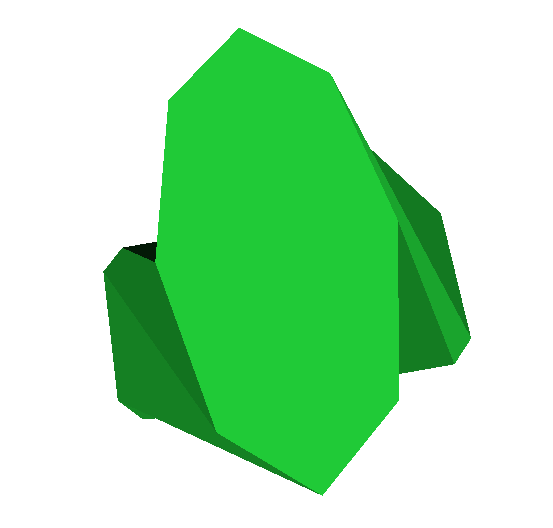
\includegraphics[width = 0.5\textwidth]{img/k3dtools-weird.png}
\caption{This is an unusual figure demonstrating the stitch operation employed on a
beveled rectangle and an octagon inscribed within an ellipse. The stitch operation
only requires that the two polygons have the same number of vertices and a polygon may
even have degenerate vertices; for example we may have an octagon which represents a point.}
\end{figure}

\begin{figure}
\label{fig:k3dtools-extrude}
\centering
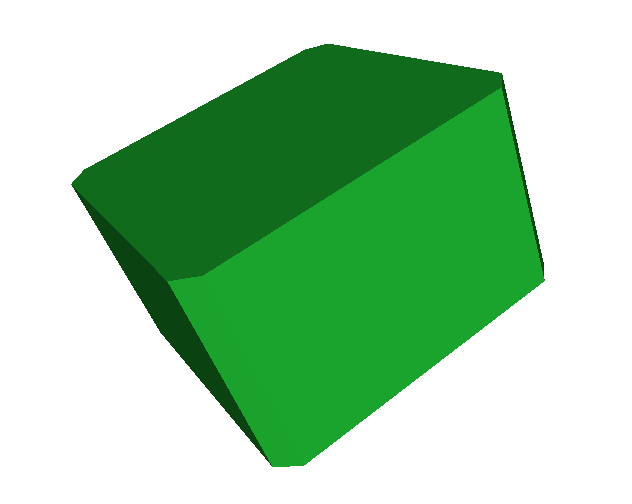
\includegraphics[width = 0.5\textwidth]{img/k3dtools-extrude.png}
\caption{A beveled polygon extruded to produce a cube.}
\end{figure}

\subsubsection{kc3d.Circle()}
\label{sec:kc3dCircle}
The \textbf{Circle} class derives from Polygon and implements a polygon of
3 to 360 vertices inscribed in an ellipse.  The more vertices, the better the approximation
to an ellipse; however, this comes at the cost of memory and file size consumed by the
model.  For an excellent representation of a circle, 48 vertices usually suffices. For
modeling small wires, 12 to 16 vertices may suffice and in some cases even 8 vertices
will produce pleasant results. The number of vertices defaults to 16 on creation
but it can be set at any time by invoking \textbf{setNVertices(n)} prior to invoking
the \textbf{calc} method to calculate the vertices.

\subsubsection{kc3d.Rectangle()}
The \textbf{Rectangle} class derives from Polygon and implements a rectangle which
may have beveled corners. The bevel can be controlled by invoking \textbf{setBevel(bevel, segments)}
before invoking the \textbf{calc} method. A bevel $\le0$ indicates the default of no bevel; segments
is a number from 1 to 360 where 1 represents a bevel and a number $>1$ represents an approximation to
a rounded corner.  The example below shows all three corner styles; it creates a green extruded
rectangle with rounded corners which has a plain black rectangular extrusion and a blue
beveled rectangular extrusion.

\begin{verbatim}
import math
import kc3d
from kc3d import *

color = VRMLMat()
color.Load("../colors/rcc_grn_g.mat")

tx = Transform()
out = ofstream()

r1 = Rectangle()
r2 = Rectangle()

r1.setBevel(1.27, 5)
r2.setBevel(1.27, 5)

r1.calc(20.32, 15, tx)

tx.setTranslation(0, 0, 1.6)
r2.calc(20.32, 15, tx)

tx.setTranslation(0,0,0)
tx.setScale(0.3937)

SetupVRML("board.wrl", out)
SetupXForm("BOARD", out, 0)

r1.paint(False, tx, color, False, out, 2)
r2.paint(True, tx, color, True, out, 2)
r1.stitch(True, r2, tx, color, True, out, 2)

r1.setBevel(0.3, 1) 
r2.setBevel(0.3, 1) 
color.Load("../colors/rcc_blu_g.mat")
tx.setScale(1)
tx.setTranslation(-5,0,1.6)
r1.calc(5, 5, tx);
tx.setTranslation(-5,0,3.6)
r2.calc(5, 5, tx);
tx.setScale(0.3937)
tx.setTranslation(0,0,0)
r2.paint(True, tx, color, False, out, 2)
r1.stitch(True, r2, tx, color, True, out, 2)

r1.setBevel(-0.3, 1) 
r2.setBevel(-0.3, 1) 
color.Load("../colors/rcc_blk_g.mat")
tx.setScale(1)
tx.setTranslation(5,0,1.6)
r1.calc(3, 3, tx);
tx.setTranslation(5,0,2.4)
r2.calc(3, 3, tx);
tx.setScale(0.3937)
tx.setTranslation(0,0,0)
r2.paint(True, tx, color, False, out, 2)
r1.stitch(True, r2, tx, color, True, out, 2)

CloseXForm(out, 0)
out.close()
\end{verbatim}

\begin{figure}
\label{fig:k3dtools-board}
\centering
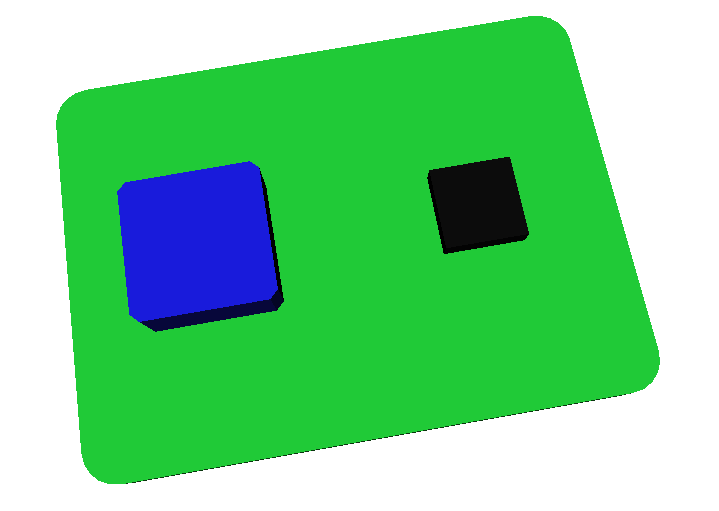
\includegraphics[width = 0.6\textwidth]{img/k3dtools-board.png}
\caption{A rectangle may be plain, as in the case of the black box, or have beveled (blue box)
or rounded corners (green board).}
\end{figure}

\subsection{kc3d.Pin()}
The \textbf{Pin} class is a representation of a vertical wire with an optional bend. The wire
may be rectangular (with or without bevels) or elliptical (see Sec.~\ref{sec:kc3dCircle} for
details about the ellipse). The starting end or both ends of the wire may be tapered, the taper
may apply to only one axis or both axes of the cross-section, and the bend may be any angle
from 0 to $\pi$ radians. 

The pin has a \textbf{calc()} method which takes a \textbf{PParams} and a Transform
argument. The members of PParams are as follows:

\begin{itemize}
\item[\textbf{w}] Pin width, X dimension\\
\item[\textbf{d}] Pin depth, Y dimension\\
\item[\textbf{h}] length of straight vertical section ($<0$ for none)\\
\item[\textbf{l}] length of straight second section ($<0$ for none)\\
\item[\textbf{bend}] bend angle, radians, $0$ to $\pi$\\
\item[\textbf{r}] bend radius, $<0$ for none\\
\item[\textbf{nb}] number of segments in a bend\\
\item[\textbf{tap}] length of tapered portion, $<0$ for none\\
\item[\textbf{dbltap}] True if both ends are to be tapered, False if only the vertical segment is tapered\\
\item[\textbf{stw}] Taper coefficient in X dimension\\
\item[\textbf{std}] Taper coefficient in Y dimension\\
\item[\textbf{bev}] bevel, applicable only to rectangular pins, $<0$ for none\\
\item[\textbf{ns}] number of vertices, applicable only to elliptical pins\\
\end{itemize}

The pin shape can be set before invoking calc via \textbf{setShape(square)} where square
is True for a rectangular pin and False for an elliptical pin; the default setting is for a
rectangular pin. The pin shape can be written to an output file via
\textbf{build(cap0, cap1, xform, color, reuse, file, tabs)} where cap0 and cap1
are booleans controlling whether or not the start and terminal ends of the pin are rendered
xform is a transformation to apply to the output data, and so on.

The example below uses two Pin objects to define the type of pin which may be found on
square pitch SMD headers:

\begin{verbatim}
import math
import kc3d
from kc3d import *

pin1 = Pin()
pin2 = Pin()

tx0 = Transform()
tx1 = Transform()
tx2 = Transform()

# set up tx0 to output to KiCAD's world scale
tx0.setScale(1.0/2.54)

# set up tx1 to lay down Pin1 and place the bottom  at Z=0
tx1.setRotation(math.pi, 1, 0, 1)
tx1.setTranslation(0, 0, 0.32)

# set up tx2 to shift the pin into position
tx2.setTranslation(4, 0, 1.32)

color = kc3d.VRMLMat()
color.Load("../colors/gold.mat")

pp0 = kc3d.PParams()
pp0.w = 0.64
pp0.d = 0.64
pp0.tap = 0.5
pp0.stw = 1
pp0.std = 0.5
pp0.dbltap = False
pp0.h = 3
pp0.r = 1
pp0.nb = 5
pp0.l = 0
pp0.bend = math.pi/2.0

pin1.calc(pp0, tx1)

pp1 = kc3d.PParams()
pp1.w = 0.64
pp1.d = 0.64
pp1.tap = -1.0
pp1.stw = 1
pp1.std = 1
pp1.dbltap = False
pp1.h = 2.44
pp1.r = 1
pp1.nb = 5
pp1.l = 5
pp1.bend = math.pi/2.0

pin2.calc(pp1, tx2)

out = kc3d.ofstream()
kc3d.SetupVRML("pindemo.wrl", out)
kc3d.SetupXForm("SMD_PIN", out, 0)
pin1.build(True, False, tx0, color, False, out, 2)
pin2.build(False, True, tx0, color, True, out, 2)
kc3d.CloseXForm(out, 0)
out.close()
\end{verbatim}

\begin{figure}
\label{fig:k3dtools-pin}
\centering
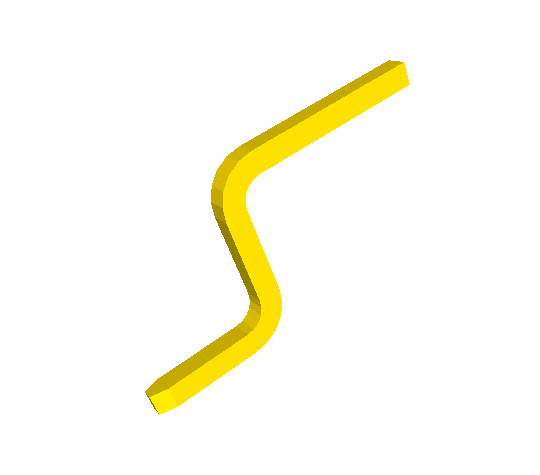
\includegraphics[width = 0.5\textwidth]{img/k3dtools-pin.png}
\caption{A pin for a typical SMD connector can be formed by superimposing
two pin objects.}
\end{figure}

\subsection{kc3d:Wire}
The class \textbf{Wire} represents a path swept with a polygon.
Vertices are added using \textbf{addPoint(q)} or \textbf{addPoint(x, y, z)}
where q is a quaternion and x, y, z represent the 3D coordinates of a point.
All points can be cleared by invoking \textbf{clear()}. The path is
rendered to a file via \textbf{build(poly, cap0, cap1, outside, tx, color, reuse, file, tabs)}
where poly is the polygon, cap0 and cap1 determine whether the ends are capped or not,
outside determines whether the wire is visible from the outside, tx is the transform
to apply to the output, color is the material appearance, reuse determines whether a
color is reused or not, file is an open output file, and tabs is the formatting
indent level.

Use wires sparingly; due to the extensive number of polygons, a wire is a costly
item. Applications of a wire include modeling an inductor and modeling the
wiring of some PCB connectors. The examples below illustrate the use of the
wire; the first example has a rectangle formed into a continuous loop with
vertices on a rectangular grid, the second shows a wire bent into an odd shape
and clearly shows how the endpoint may change orientation depending on how the
wire is bent.  The third example is a triangular helical coil; a close look at
the wire ends will reveal a change in orientation; setting the number of
vertices of the circle to 3 (triangle) rather than 8 will make the change in
orientation more obvious. Note how much memory is consumed by the coil model;
a more realistic coil model would have perhaps 24 vertices in a single twist
of the helix and would take approximately 8 times as much memory.

\begin{verbatim}
import math
import kc3d
from kc3d import *

color = VRMLMat()
color.Load("../colors/rcc_grn_g.mat")

w = Wire()
w.setParams(8,1.0)
r = Rectangle()
t0 = Transform()

r.setBevel(0.1, 1)
r.calc(1, 1, t0)

out = ofstream()
SetupVRML("wiredemo_A.wrl", out)
SetupXForm("WIRE_DEMO", out, 0)
# last leg is rendered from the wrong side
w.addPoint(0, 0, 1)
w.addPoint(0, 0, 4)
w.addPoint(4, 0, 4)
w.addPoint(4, -4, 4)
w.addPoint(0, -4, 4)
w.addPoint(0, -4, 0)
w.addPoint(4, -4, 0)
w.addPoint(4, 0, 0)
w.addPoint(1, 0, 0)
w.addPoint(0, 0, 0)
w.addPoint(0, 0, 1)
w.build(r, False, False, True, t0, color, False, out, 2)
w.clear()
CloseXForm(out, 0)
out.close()

SetupVRML("wiredemo_B.wrl", out)
SetupXForm("WIRE_DEMO", out, 0)
w.addPoint(0, 0, 0)
w.addPoint(0, 0, 4)
w.addPoint(4, 0, 4)
w.addPoint(4, -4, 4)
w.addPoint(0, -4, 4)
w.addPoint(1, -3, 0)
w.addPoint(4, -4, 0)
w.addPoint(4, -4, -3)
w.build(r, True, True, True, t0, color, False, out, 2)
w.clear()
CloseXForm(out, 0)
out.close()


# Triangular spiral
color.Load("../colors/copper.mat")
c = Circle()
c.setNVertices(8)
c.calc(1.0, 1.0, t0)
# Lead in
w.addPoint(0, 0, -5)
w.addPoint(0, 0, 0)
# Spiral
x = 1.0/3.0;
h = math.sqrt(75.0)
while x < 10:
    w.addPoint(x, 5, 0)
    x += 1.0/3.0
    w.addPoint(x, 0, h)
    x += 1.0/3.0
    w.addPoint(x, -5, 0)
    x += 1.0/3.0

# Lead out
w.addPoint(x, 0, 0)
w.addPoint(x, 0, -5)
SetupVRML("wiredemo_C.wrl", out)
SetupXForm("WIRE_DEMO", out, 0)
w.build(c, True, True, True, t0, color, False, out, 2)
w.clear()
CloseXForm(out, 0)
out.close()
\end{verbatim}

\begin{figure}
\label{fig:k3dtools-coil}
\centering
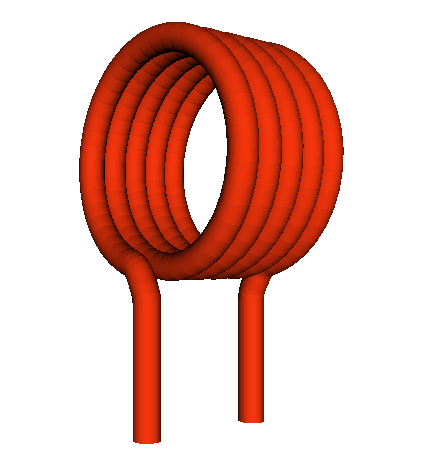
\includegraphics[width = 0.5\textwidth]{img/k3dtools-coil.png}
\caption{The wire model can be used to create objects such as an inductor. Care must be taken
when using the wire model because the resulting file may be very large; the model shown
has a file size of almost 2MB.}
\end{figure}

\subsection{kc3d.Funnel()}
The \textbf{Funnel} class is a representation of a rectangular or elliptical funnel typical
of the pin recesses in a connector. The default shape of the funnel is rectangular but the
shape can be set by invoking \textbf{setShape(square, bevel)} where \textbf{square} is True for
a rectangular funnel and \textbf{bevel} is the bevel to use on the rectangular section; use
a bevel value $<0$ for a plain rectangle.

The vertices are calculated by invoking \textbf{calc(w1, d1, w2, d2, h1, h2, h3, xform, ns)}
where w1 and d1 are the X and Y dimensions of the top of the flute, w2 and d2 and the
dimensions of the stem, h1 is the height of the flute, h2 is the height of the segment of
the stem which is the same color as the flute (this may be set to 0), and h3 is the
height of the stem segment which will be colored with stemcolor.

The shape is written to an output file by invoking \textbf{build(cap, xform, flutecolor,
reuse\_flute, stemcolor, reuse\_stem, file, tabs)} where cap is a boolean controlling
whether or not the bottom end of the stem is rendered, flutecolor is a VRMLMat object
specifying the color of the flute and the stem segment h2, reuse\_flute is a boolean
controlling the reuse of flutecolor, stemcolor is a VRMLMat object specifying the color
of the h3 section of the stem, and reuse\_stem controls the reuse of the stem color.

The example below creates a funnel with a blue beveled flute and golden stem:

\begin{verbatim}
import kc3d
from kc3d import *

tx = Transform()

fun = Funnel()
fun.setShape(True, 0.2)
fun.calc(1.6, 1.6, 0.96, 0.96, 0.5, 0.2, 3, tx, 24)

fcolor = kc3d.VRMLMat()
fcolor.Load("../colors/rcc_blu_g.mat")

scolor = kc3d.VRMLMat()
scolor.Load("../colors/gold.mat")

out = kc3d.ofstream()
kc3d.SetupVRML("funneldemo.wrl", out)
kc3d.SetupXForm("FUNNEL_DEMO", out, 0)
fun.build(True, tx, fcolor, False, scolor, False, out, 2)
kc3d.CloseXForm(out, 0)
out.close()
\end{verbatim}

\begin{figure}
\label{fig:k3dtools-funnel}
\centering
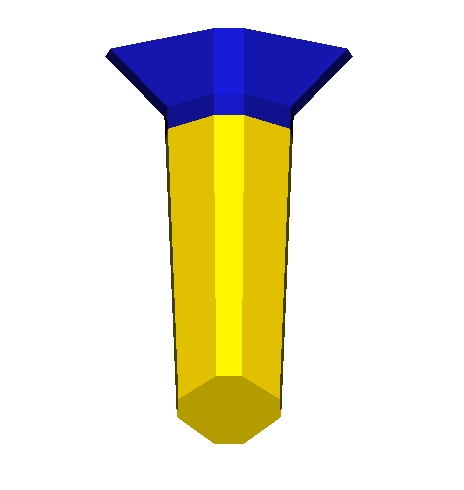
\includegraphics[width = 0.5\textwidth]{img/k3dtools-funnel.png}
\caption{A square funnel typical of female header connectors. The funnel model
can also produce circular funnels and more esoteric shapes such as rectangular
and elliptical funnels.}
\end{figure}

\subsection{kc3d.Hole()}
The \textbf{Hole} class represents a plain rectangular panel with a rectangular or elliptical
hole in it; a rectangular hole may be beveled. A hole may be used to surround the flute of a
funnel or to provide thru-holes for pins.

The vertices are calculated by invoking \textbf{calc(w1, d1, w2, d2, tx, square, off\_x, off\_y, np, bev)}
where w1 and d2 are the X and Y dimensions of the frame, w2 and d2 are the dimensions of the
hole, square specifies a rectangular hole when set to True, off\_x and off\_y are offsets of
the hole, np is the number of vertices in a circular hole and bev is the optional bevel of
a rectangular hole (set bev to -1 if you do not want a bevel).

The shape information is written to a file by invoking \textbf{build(xform, color, reuse, file, tabs)}.

\subsection{kc3d.Shoulder()}
The \textbf{Shoulder} class represents a rectangular extrusion which may have one rounded edge
and which may have ends which taper. A shoulder may be found, for example, as a spacer on the
bottom of header cases.

Vertices are calculated by invoking \textbf{calc(l, h, w, t, r, xform)} where l and h are the length
and height of the shoulder, w is the depth, and r is the radius of the lower inner edge ($<0$ for no radius).

The shape information may be written by invoking \textbf{build(xform, color, reuse, file, tabs)}.

\subsection{kc3d.Hdrbase()}
The \textbf{Hdrbase} class is a generic case for a square-pitch header. The case is rectangular but
may be beveled between each column of pins, the holes for the pins may be square or circular, the
holes may be a different size on the top and bottom, and the part may have a rectangular shoulder.

Case parameters are specified by invoking \textbf{setParams(xpitch, ypitch, bevel, height, sh, hassh, hd0,
hdy, hd1, squarebot, squaretop, male, pbev, fbev, columns, rows, ns)}:

\begin{itemize}
\item \textbf{xpitch}: pin pitch along the X axis (columns)
\item \textbf{ypitch}: pin pitch along the Y axis (rows)
\item \textbf{bevel}: bevel between columns ($<0$ for none)
\item \textbf{height}: overall height of the case (measured from the top of the PCB)
\item \textbf{sh}: shoulder height ($<0$ for none); this is the gap between the top of the PCB and the bottom of the header
\item \textbf{hassh}: set True if a shoulder is to be rendered; otherwise the sh parameter simply produces a gap
\item \textbf{hd0}: X dimension of the bottom hole (if the hole is circular, the Y dimension will be set equal to hd0)
\item \textbf{hdy}: Y dimension of the bottom hole; applicable only if the hole is rectangular
\item \textbf{hd1}: dimension of the top hole; the top hole is constrained to a square or circle if the case type is
    for a female header and if the case is for a male header the top hole dimensions are the same as the bottom
    hole dimensions
\item \textbf{squarebot}: set True if the bottom pins are square or rectangular
\item \textbf{squaretop}: set True if the top holes are square (applicable only for female headers)
\item \textbf{male}: set True if the case is for a male header
\item \textbf{pbev}: bevel of the bottom hole; applicable only if squarebot is True
\item \textbf{fbev}: bevel of the top hole; applicable only if male is False and squaretop is True
\item \textbf{columns}: number of columns; valid range is $\ge1$
\item \textbf{rows}: number of rows; valid range is $\ge1$
\item \textbf{ns}: number of vertices to use for circular pins
\end{itemize}

The shape information is written to a file by invoking \textbf{build(xform, color, reuse, file, tabs)}.
The example below creates a beveled 6x2 header case suitable for a vertical female header with square pins.
Notice that the case does not include any features such as a funnel on the top holes since such features
are specific to individual header models; for example the Genhdr model may place one of at least three
different features into the top holes.

\begin{verbatim}
import kc3d
from kc3d import *

hdr = Hdrbase()
tx0 = Transform()

# set up tx0 to output to KiCAD's world scale
tx0.setScale(1.0/2.54)

color = kc3d.VRMLMat()
color.Load("../colors/rcc_blu_g.mat")

hdr.setParams(2.54, 2.54, 0.3, 8, 0.72, True, 0.64, 0.64, 1.6, True, True, False, -1, -1, 6, 2, 24)

out = kc3d.ofstream()
kc3d.SetupVRML("hdrcasedemo.wrl", out)
kc3d.SetupXForm("HEADER_CASE_DEMO", out, 0)
hdr.build(tx0, color, False, out, 2)
kc3d.CloseXForm(out, 0)
out.close()
\end{verbatim}

\begin{figure}
\label{fig:k3dtools-hdrcase}
\centering
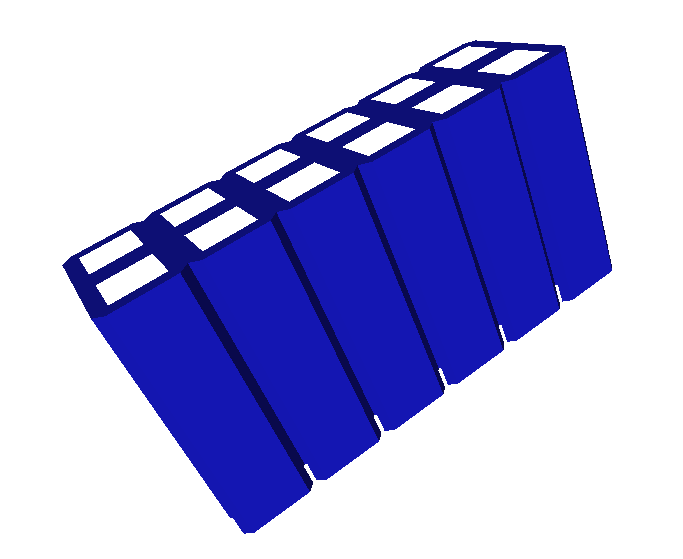
\includegraphics[width = 0.6\textwidth]{img/k3dtools-hdrcase.png}
\caption{A sample of a header casing suitable for a female header connector.
The multiple holes on the top are rendered by the Hole object.}
\end{figure}


\section{KC3DCONN: The Connector Toolbox}
The module \textbf{kc3dconn} contains parametric models
of connectors.  We have already seen an example of such
a model in Section~\ref{sec:quick-example}.

\subsection{kc3dconn:Genhdr}
The class \textbf{Genhdr} represents a generic square-pitch vertical header.
The header may have square or circular pins, may be male or female, may
have a plain or beveled casing, and may have a shoulder on the casing.
Section~\ref{sec:quick-example} presented this class and demonstrated its
use although no details were discussed. Internally the class makes use of
the classes \textbf{VRMLMat}, \textbf{Hole}, \textbf{Hdrbase}, \textbf{Pin},
\textbf{Funnel}, and \textbf{Circle} to generate all the features of the
header.

The parameters controlling the final appearance of the header have been
divided into a number of groups: Color parameters, Case parameters, and
Pin parameters.

The colors can be selected by invoking \textbf{setColors(case, pin\_out, pin\_in, shroud)}
where each argument is of type VRMLMat, case is the color of the case, pin\_out is the outer
appearance of the pin, and pin\_in is the inner appearance of the pin, and shroud is the appearance of
the recess or protrusion around a pin; pin\_out and shroud are applicable only
to female headers.

The case parameters are set via \textbf{setCase(columns, rows, col\_pitch, row\_pitch, height, shoulder, hassh, bevel)}
where height is the total case height, shoulder is the height of the case shoulder, and bevel is the
case bevel between columns. The parameter hassh controls whether a shoulder is rendered (True) or if the shoulder
parameter simply specifies a gap between teh PCB and the case (False).

The pin parameters are set via
\textbf{setPins(squarebot, squaretop, male, pbev, fbev, depth, length, pd0, pdy, pd1, pd2, pd3, ftc, taper, ts, sides, funneldepth)}:

\begin{itemize}
\item \textbf{squarebot}: set True if the pin is square or rectangular
\item \textbf{squaretop}: set True if the receptacle is square (applicable only to female headers)
\item \textbf{male}: set True if the header is male
\item \textbf{pbev}: pin bevel; applicable only if squarebot is True
\item \textbf{fbev}: funnel bevel; applicable only if male is False and squaretop is True
\item \textbf{depth}: pin length below the top of the PCB
\item \textbf{length}: total pin length (depth + total connector height above PCB)
\item \textbf{pd0}: X dimension of pins
\item \textbf{pdy}: Y dimension of pins; applicable only if squarebot is True
\item \textbf{pd1}: dimension of the shroud around the receptacle; applicable only when male is False
\item \textbf{pd2}: inner dimension of the receptacle; applicable only when male is False
\item \textbf{pd3}: diameter of the pin where it enters the bottom of the casing; applicable only when
    male and squarebot are False
\item \textbf{ftc}: when male and squaretop are False, ftc controls the bevel at the receptacle's entrance;
    valid values are $\ge1$.
\item \textbf{taper}: pin taper length (set to $\le0$ for none
\item \textbf{ts}: taper coefficient; controls the size of the tapered end
\item \textbf{sides}: number of vertices to use for circular pins or receptacles
\item \textbf{funneldepth}: for a square receptacle this is the depth of the funnel's flute and must be $\ge0$;
    for a circular receptacle this is the depth of the recess ($>0$), the height of the protrusion ($<0$),
    or 0 for a receptacle which is flush with the housing.
\end{itemize}

Genhdr has been used to create models for Samtec headers in series SS, HSS, ESS, SD, ESD, SL, and SLD
and can be used to generate models for headers from many other manufacturers.


\section{KC3DRES: The Resistor Toolbox}
The module \textbf{kc3dres} represents parametric models of resistors. 

\subsection{kc3dres:Resistor}
The class \textbf{Resistor} represents a thru-hole cylindrical resistor such as
the typical color-coded Carbon Composite Resistor or Metal Film Resistor. The
resistor model itself is generated by a simple command, in the example below it is
\verb#R.create(P, "11X55X66X22XXGG", "resistordemo")#, however the model takes
about 28 parameters which need to be set up beforehand.  The parameters are all
stored in the structure \textbf{kc3dres.RParams} and are as follows:

\begin{itemize}
\item\textbf{scale}: scale factor to apply to final result
\item\textbf{shift}: shift along X-axis to center reference point (usually 1/2 pitch)
\item\textbf{L}: length of resistor body
\item\textbf{D}: diameter of resistor body
\item\textbf{d}: diameter of wire
\item\textbf{p}: lead pitch
\item\textbf{wl}: wire length below top of PCB
\item\textbf{horiz}: True for horizontal orientation
\item\textbf{endshape}: resistor end style, `C'ap, `R'ound, or `B'ulge (default)
\item\textbf{bcap}: True if a Bulge style body also has metallic end caps
\item\textbf{wsides}: number of vertices in a wire cross-section
\item\textbf{bsides}: number of segments in a right angle bend
\item\textbf{rsides}: number of vertices in the resistor body cross-section
\item\textbf{pwrsuf}: optional suffix to indicate power rating, ex: ``0W25''
\item\textbf{spcsuf}: optional suffix to indicate lead spacing and orientation, ex: ``0I40H''
\item\textbf{colors}: colors mapped to the color code, body color, wire color
\end{itemize}

The \textbf{colors} parameters cannot be accessed directly; use the helper function
\textbf{setRColors(index, params, colorfile)} to set the colors. The indices are
0 to 9 to represent the code for the digits 0 to 9, 10 for gold, 11 for silver,
12 for the body color, and 13 for the wire color.

To create the 3D model, set up the parameters and then invoke
\textbf{create(params, code\_string, base\_name)} where params is the
set of parameters previously set up, code\_string is a string representing
the colored bands and gaps, and base\_name is the base filename; the
routine will add the endstyle code, power suffix, lead space suffix, and the
suffix ``.wrl'' to produce the full file name. The recommended format for the
base name is \textbf{[Part Series]\_[Value]\_[Tolerance][T coeff]}, for example
``CCR\_11R\_J-'' is a generic carbon composite (part series) with $11\Omega$
resistance, tolerance class J, with no specified temperature coefficient.
The code string is a series of characters from the set 0..9, G, S, X and
each character represent a band on the resistor. Repeat characters as
necessary to obtain the required band widths and spacings; you may even
add a temperature coefficient band. In the example below, the string
``11X55X66X22XXGGG'' represents an imaginary 15.6K resistor with $5\%$
tolerance; the tolerance band is 1.5 times the width of a value band.
As an example of the flexibility of this coding system, you can specify
a $0\Omega$ link with the code ``XXX0XXX''.

A wide variety of resistors (Series E96 + E24 for 0.5W 1\% MFR, Series E48
for 0.5W 2\% MFR, Series E24 for 0.25W 5\% CCR) have been rendered in
horizontal orientation with 0.4 inch lead spacing and in vertical
orientation with 0.2 inch lead spacing, so this module is most useful
for generating models which are not already available. The necessary
scripts and modules also take up much less storage space than the
pre-generated models so in the future the pre-generated models may
be discontinued and models may be generated via script as needed.

\begin{verbatim}
import kc3d
import kc3dres
from kc3d import *
from kc3dres import *

R = Resistor()
P = RParams()

# load the colors for the resistor codes, body, and wires
setRColors(0, P, "../colors/rcc_blk_g.mat")
setRColors(1, P, "../colors/rcc_brn_g.mat")
setRColors(2, P, "../colors/rcc_red_g.mat")
setRColors(3, P, "../colors/rcc_org_g.mat")
setRColors(4, P, "../colors/rcc_yel_g.mat")
setRColors(5, P, "../colors/rcc_grn_g.mat")
setRColors(6, P, "../colors/rcc_blu_g.mat")
setRColors(7, P, "../colors/rcc_pur_g.mat")
setRColors(8, P, "../colors/rcc_gry_g.mat")
setRColors(9, P, "../colors/rcc_wht_g.mat")
setRColors(10, P, "../colors/rcc_gld_g.mat")
setRColors(11, P, "../colors/rcc_slv_g.mat")
setRColors(12, P, "../colors/rbc_blu_g.mat")
setRColors(13, P, "../colors/tin.mat")

# set the resistor parameters
P.scale = 0.3937
P.shift = -2.54
P.L = 6.3
P.D = 2.3
P.d = 0.6
P.wl = 2.0
P.p = 5.08
P.horiz = False
P.endshape = 'B'
P.bcap = True
P.wsides = 16
P.bsides = 5
P.rsides = 48
P.pwrsuf = "0W50"
P.spcsuf = "0I20"

R.create(P, "11X55X66X22XXGGG", "resistordemo")
\end{verbatim}


\begin{figure}
\label{fig:k3dres-horiz}
\centering
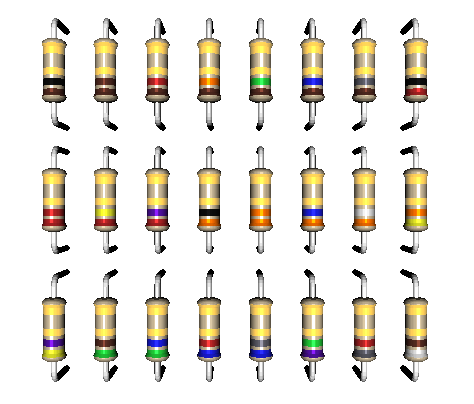
\includegraphics[width = 0.5\textwidth]{img/k3dres-horiz.png}
\caption{Sample of first decade of horizontal carbon composite resistors,
0.4 inch pitch, series E24, 0.25W, 5\% tolerance.}
\end{figure}

\begin{figure}
\label{fig:k3dres-vert}
\centering
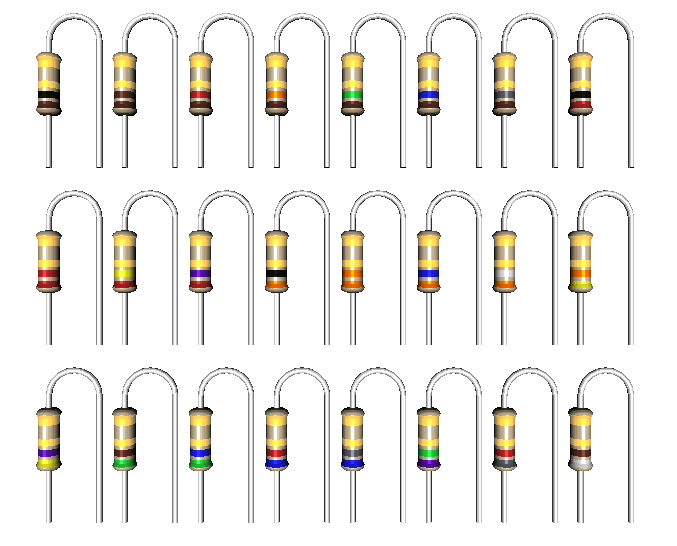
\includegraphics[width = 0.5\textwidth]{img/k3dres-vertical.png}
\caption{Sample of first decade of vertical carbon composite resistors,
0.2 inch pitch, series E24, 0.25W, 5\% tolerance.}
\end{figure}


\subsection{kc3ddip:Dip}
The class \textbf{Dip} represents a thru-hole DIL package. The general
case parameters are set by invoking the member function \textbf{setParams(params)} where
params is a DipParams object with the following members:

\begin{itemize}
\item\textbf{A1} height from top of PCB to bottom of case\\
\item\textbf{A2} height of case\\
\item\textbf{L} depth of pin from top of PCB\\
\item\textbf{e} pin pitch\\
\item\textbf{E} row spacing\\
\item\textbf{E1} case width\\
\item\textbf{B1} wide portion of pin\\
\item\textbf{b} narrow portion of pin\\
\item\textbf{c} pin thickness\\
\item\textbf{NW} notch width (nominal 0.06 inch)\\
\item\textbf{ND} notch depth (nominal 0.012 inch)\\
\item\textbf{NL} notch length (nominal 0.07 inch, must be $>\textrm{ND}$)\\
\item\textbf{casebev} bevel on case (nominal 0.005 inch)\\
\item\textbf{pinbev} bevel on pin (nominally $\textrm(c)/10$)\\
\item\textbf{MID} height of middle case portion where pin attaches (nominally $1.4*\textrm{c}$);
    set to a negative number to default to the nominal value\\
\item\textbf{DW} extra length on case (nominal $2*(\textrm{c}/3 + \textrm{B}1/2)$);
    set to a negative number to default to the nominal value\\
\item\textbf{S} deviation of unbeveled top and bottom edged from mid section (taper);
    set to a negative number to default to the nominal value (5 degree taper)\\
\item\textbf{scale} scale factor to apply to final output\\
\end{itemize}


The remaining Dip class member functions are as follows:

\textbf{setPins(npins)} sets the nominal number of pins to npins; npins must
be $\ge4$ and must be a multiple of 2. The nominal number of pins is used in
calculating the total length of the package. The nominal number is the maximum
number of pins which can be attached to the package; the pins which are
actually rendered are controlled via the \textbf{setPin()} function.
Return values are 0 for success and -1 for failure.

\textbf{setPin(pin, on)} selects whether a specific pin should be rendered or
not. By default all pins are rendered unless this routine is invoked to suppress
a pin. Return values are 0 for success and -1 for failure.

\textbf{setPinColor(filename)} and \textbf{setCaseColor(filename)} load
a material appearance file for the pin and case. These functions return 0
for success and -1 for failure.

\textbf{create(filename)} calculates the model features and writes the
result to the specified filename. Return values are 0 for success and -1 for failure.

The example below creates two DIL-12 packages; one has a complete set of pins while
the other only has the 2 pins in each corner. This demonstrates how the software
can be used to generate typical DIP models as well as specialised models, such as
packaged reed relays, which may be missing pins.

\begin{verbatim}
import kc3ddip
from kc3ddip import *

# the parameters are initialized to suit 0.3" pitch
p = DipParams()


dil = Dip()
dil.setParams(p)
dil.setPins(12)
# we need to specify colors
dil.setPinColor("../colors/tin.mat")
dil.setCaseColor("../colors/ceram_gry.mat")

# write out the normal DIP
dil.create("DIL_12_plain.wrl")

# suppress pins; note that pins are numbered from 1..N
dil.setPin(3, False)
dil.setPin(4, False)
dil.setPin(9, False)
dil.setPin(10, False)

# write out the special DIP
dil.create("DIL_12_special.wrl")
\end{verbatim}





\section{KC3DDIODE: The Diode Toolbox}
The module \textbf{kc3ddiode} contains parametric models
of diodes. The models are as follows:

\begin{itemize}
\item \textbf{do35}: DO-35 package glass encapsulated axial diode
\item \textbf{GenDiode}: Generic tubular axial diode
\end{itemize}

\subsection{kc3ddiode:do35}
The class \textbf{do35} represents a DO-35 package glass encapsulated
axial diode such as the 1N4148. Most parameters are fixed according
to the DO-35 specification but the user has some control of the
material appearance, lead pitch, and orientation. The dimensions used
are the Maximum Material Condition specifications. The public methods
include:

\textbf{setColors(wirecolor, glasscolor, cathodecolor, tubecolor)}
where the arguments are the filenames for material appearance specifications
(VRMLMat files). The wirecolor controls the appearance of the lead,
glasscolor controls the appearance of the glass envelope,
cathodecolor controls the appearance of the cathode band, and
tubecolor controls the appearance of the metallic tube inside the
glass envelope.

\textbf{setNVertices(wire, tube, bend)} where wire is the number of
vertices to use for the wire's cross-section, tube is the number of
vertices to use in the cross-section of the envelope and tube,
and bend is the number of segments in a bend.

\textbf{build(partname, scale, horiz, vflip, pitch, lead)}: create the
3D model; partname is the name of the part and also the base name of the
output file; it must contain only the characters a..z, A..Z, 0..9, and the 
underscore character and the first character must be an alphabetic character.
scale is the scale factor; since the internal units are in mm, use a scale of
0.3937 to produce a model for use in the KiCAD 3D viewer. horiz must be set to
True for horizontal orientation; when the orientation is vertical, vflip may
be set to True to place the cathode at pin 2. pitch is the lead pitch and
lead is how far the lead protrudes below the top of the PCB.

The example below creates a DO-35 package diode in a horizontal orientation,
in which the cathode is always pin 1, and in two vertical orientations in which
the cathode is first on pin 1 and then on pin 2.

\begin{verbatim}
import kc3d
from kc3d import *
import kc3ddiode
from kc3ddiode import *

diode = do35()
diode.setNVertices(16, 48, 5)
diode.setColors("../colors/tin.mat", "../colors/glass_clr.mat",
    "../colors/glass_blk.mat", "../colors/copper.mat")

# horizontal with 0.3" pitch; the cathode is always pin 1
diode.build("do35_0I300H", 0.3937, True, False, 7.62)

# we must double the number of bend segments in the
# vertical orientation since we have a 180 degree bend
# rather than 90 degree bends:
diode.setNVertices(16, 48, 10)

# vertical with 0.1" pitch, the cathode is pin 1
diode.build("do35_0I100V", 0.3937, False, False, 2.54)

# vertical with 0.1" pitch, the cathode is pin 2
diode.build("do35_0I100VK2", 0.3937, False, True, 2.54)
\end{verbatim}




\subsection{kc3ddiode:GenDiode}
The class \textbf{GenDiode} represents a generic tubular axial diode;
the model has been used to generate 3D models of diodes with the
DO-41, DO-201, and DO-204 package specifications. Since the dimensions
are not hard-coded as in the case of the do35 model, the output is
not strictly limited to the Maximum Material Condition of any particular
package specification. The public methods
include:

\textbf{setColors(wirecolor, bodycolor, cathodecolor)}
where the arguments are the filenames for material appearance specifications
(VRMLMat files). The wirecolor controls the appearance of the lead,
bodycolor controls the appearance of the envelope, and
cathodecolor controls the appearance of the cathode band.

\textbf{setNVertices(wire, tube, bend)} where wire is the number of
vertices to use for the wire's cross-section, tube is the number of
vertices to use in the cross-section of the envelope and tube,
and bend is the number of segments in a bend.

\textbf{build(partname, scale, horiz, vflip, pitch, lead)}: create the
3D model; partname is the name of the part and also the base name of the
output file; it must contain only the characters a..z, A..Z, 0..9, and the 
underscore character and the first character must be an alphabetic character.
scale is the scale factor; since the internal units are in mm, use a scale of
0.3937 to produce a model for use in the KiCAD 3D viewer. horiz must be set to
True for horizontal orientation; when the orientation is vertical, vflip may
be set to True to place the cathode at pin 2. pitch is the lead pitch and
lead is how far the lead protrudes below the top of the PCB.

\textbf{setParams(wire, body, length, band, space)}: set the dimensions of the
package; wire is the wire diameter, body is the tube (body) diameter, length
is the tube's length, band is the width of the cathode band, and space is the
distance between the edge of the tube and the diode band.

The example below creates a DO-41 package diode in Maximum Material Condition
in a horizontal orientation and two vertical orientations:

\begin{verbatim}
# load the tools
import kc3d
import kc3ddiode
from kc3d import *
from kc3ddiode import *

diode = GenDiode()
diode.setNVertices(16, 48, 5)
#DO41 has max material for dwire = 0.864, dbody = 2.72, lbody = 5.21
diode.setParams(0.864, 2.72, 5.21, 0.8, 0.6)
diode.setColors("../colors/tin.mat", "../colors/rcc_blk_g.mat", "../colors/rcc_wht_g.mat")

# horizontal orientation (pin 1 is always the cathode)
diode.build("do41_0I400H", 0.3937, True, False, 10.16)

diode.setNVertices(16, 48, 10)

# vertical orientation, pin 1 is the cathode
diode.build("do41_0I100V", 0.3937, False, False, 2.54)

# vertical orientation, pin 2 is the cathode
diode.build("do41_0I100VK2", 0.3937, False, True, 2.54)
\end{verbatim}


\end{document}
